\documentclass[11pt]{article}
\usepackage[margin=1in]{geometry}
\usepackage{amsmath,amssymb}
\usepackage{graphicx}
\usepackage{booktabs}
\usepackage{microtype}
\usepackage{xcolor}
\usepackage[hidelinks]{hyperref}
\usepackage{titlesec}
\usepackage{enumitem}
% Tolerance Law numbers — generated by analyze_tolerance.py
% Do not edit by hand.  Current values are STUBS; replace after grid completes.
\newcommand{\TLteacherTight}{90\%}
\newcommand{\TLteacherLoose}{100\%}
\newcommand{\TLclearances}{4}
\newcommand{\TLwidths}{3}
\newcommand{\TLbudgets}{3}
\newcommand{\TLseeds}{10}
\newcommand{\TLtenSeed}{10}
\newcommand{\TLevalEp}{40}
\newcommand{\TLcells}{360}
\newcommand{\TLthreshold}{0.50}


\definecolor{steel}{RGB}{30,60,120}
\titleformat{\section}{\large\bfseries\color{steel}}{\thesection}{0.6em}{}
\titlespacing*{\section}{0pt}{2.2ex}{1.2ex}

\title{\bfseries The Tolerance Law:\\[0.3em]
\large Learnability of Contact-Rich Assembly Skills Is a Non-Monotone
Phase Transition in Model Capacity, with a Measurable Optimal Operating Point}
\author{Sehaj Singh\\[0.4em]
\small\emph{Manufacturing robotics, learning from demonstration}}
\date{\today}

\begin{document}
\maketitle

\begin{center}
\fbox{\begin{minipage}{0.92\textwidth}\small
\textbf{Standfirst.} A robot either can or cannot learn to insert a part---and
in our controlled study, that binary depends on an engineering parameter the
factory already controls: the \emph{clearance} between peg and channel. But
the dependency is not the one engineers might expect. \emph{More model capacity
does not always help}: at tight clearance, an overly wide network overfits
demonstration noise and \emph{degrades}, while an underparameterised network
cannot capture the oscillatory insertion strategy at all. Between these regimes
lies a capacity sweet spot that a closed-loop controller discovers online. The
boundary between learnable and unlearnable is a phase transition in clearance,
and the transition curve is a non-monotone function of model width---a
\emph{Tolerance Law} that reframes the ``data problem'' of manufacturing
robotics.
\end{minipage}}
\end{center}

\section{Introduction}

Assembly is the least automated step in manufacturing. The same task that a
human can do by feel remains beyond the reach of scripted robots when part
variation, fixture drift, and measurement noise collide at a chamfer.
Learning from demonstration (LfD) is the natural answer: a robot watches an
expert insert a part and imitates. Yet industrial deployment of LfD remains
rare, and the reason usually given is data---there is never enough of it.

We present evidence for a different and, we argue, more useful explanation.
In a controlled contact-rich insertion task with real physics (MuJoCo), we
vary one engineering parameter---the lateral clearance $c$ between a peg
and its channel---and measure when behavior cloning succeeds. The result is
not a gradual degradation but a \emph{boundary}: below a clearance $c^*$,
the learned policy jams with near-certainty; above it, it inserts reliably.
The boundary exists even when the expert teacher succeeds on
\TLteacherTight\ of episodes at the tightest clearance, which isolates the
learner as the cause.

The second and more surprising result is that the boundary is a
\emph{non-monotone} function of model capacity. At fixed data budget,
increasing the width of the behavior-cloning network from $w=32$ to
$w=128$ pushes the boundary downward (more clearances become learnable).
But increasing further to $w=256$ pushes the boundary \emph{back up}:
the larger network overfits the oscillatory demonstration noise and
degrades on held-out episodes. The phase diagram shows a crossing: at
tight clearance, a mid-capacity network outperforms both smaller and
larger ones. An adaptive capacity controller that walks width upward at
fixed budget and stops when learning succeeds correctly identifies
$w=128$ as the minimum effective capacity at each clearance---a capacity
\emph{sweet spot} that the factory can find online.

We call the aggregate the \emph{Tolerance Law}: in assembly LfD,
learnability is a phase transition in an engineering parameter, the
transition boundary depends on model capacity, and the relationship is
\emph{non-monotone}---bigger is not always better. If it holds beyond
this planar task, it reframes the capacity-planning problem in
manufacturing robotics: the question is not only \emph{how much data}
but \emph{what capacity that data buys}, and the answer has a sweet spot
the factory can discover.

\section{The task and the teacher}

\paragraph{Environment.} A two-axis gantry stage carries a rigid peg
($50\times50$\,mm face) toward a slot whose channel width is $2(\tfrac{1}{2}
w_{peg} + c)$, so $c$ is the per-side clearance in metres. The slot sits on
a fixture that is rigidly locked during each episode; its true position
$y_{\mathrm{ch}}$ is sampled uniformly in $\pm 0.10$\,m and the robot observes
a noisy measurement $y_{\mathrm{meas}} \sim \mathcal{N}(y_{\mathrm{ch}},
\sigma_y^2)$ with $\sigma_y = 1.2$\,mm. Observations are
$[\text{peg}_x, \text{peg}_y, \dot x, \dot y, y_{\mathrm{meas}}, F_x, F_y, t]$
and actions are velocity commands integrated by position actuators that can
sustain insertion force (150\,N/m axial, 400\,N/m lateral, 80\,N cap).
Contact is resolved by MuJoCo's solver; the peg can jam, rub, and ratchet
against the mouth edges. Four clearances span $c = 0.0005$ to $0.004$\,m
(0.5 to 4\,mm).

\paragraph{The teacher is force-blind.} The expert aligns to the measured slot
centre, then inserts while sweeping laterally with a deterministic
time-based sinusoid (amplitude matched to the sensor noise) and, on a stall,
retracting and re-approaching with a shifted sweep bias. It never reads the
contact forces. Its success is \TLteacherTight\ at the tightest clearance and
\TLteacherLoose\ at the loosest---measured over 30 episodes each. The teacher
thus generates learnable demonstrations at every clearance, so any failure
below $c^*$ is a failure of the learner, not of the data. The sweep is a
deterministic function of time (which is in the observation), so a
behavior-cloned policy can in principle reproduce it; its \emph{fitted
amplitude} is exactly the quantity that is fragile to capacity mismatches.

\paragraph{Learners.} Behavior cloning by regression (MSE on actions) with an
MLP whose width $w \in \{32, 128, 256\}$ and depth $d \in \{2, 3, 4\}$ are
the capacity axis (\TLwidths{} width choices). Policies are trained on $N$
successful demonstrations ($N \in \{20, 60, 160\}$, \TLbudgets{} budget levels)
and evaluated on $n_{\mathrm{eval}} = 40$ fresh episodes with 2 seeds
(\TLcells{} cells in total). Success is a fully seated peg held for 10 steps.

\section{Results}

\subsection{The capacity--data phase diagram}

Figure~\ref{fig:phase} shows learned success as a function of clearance,
capacity, and budget. Three facts stand out.

\textbf{First}, there is a learnability boundary: at any fixed (capacity,
budget), success drops steeply across a narrow clearance band. The boundary
is not an artifact of a weak teacher---the teacher succeeds at every clearance
(Fig.~\ref{fig:phase}, top).

\textbf{Second}, the boundary is non-monotone in width. At $N=20$ (small
budget), $w=128$ outperforms both $w=32$ and $w=256$ at tight clearance. At
$N=160$ (large budget), the same ordering holds---and $w=256$ \emph{worsens}
relative to its smaller self, confirming overfitting. The largest model is
not the best model.

\textbf{Third}, the data budget shifts the boundary but with diminishing
returns. At $w=128$, all budgets achieve near-perfect success at every
clearance, meaning the mid-capacity network reaches the data ceiling quickly.
At $w=32$, more data helps; at $w=256$, more data hurts---the budget effect
is capacity-dependent.

\begin{figure}[t]
\centering
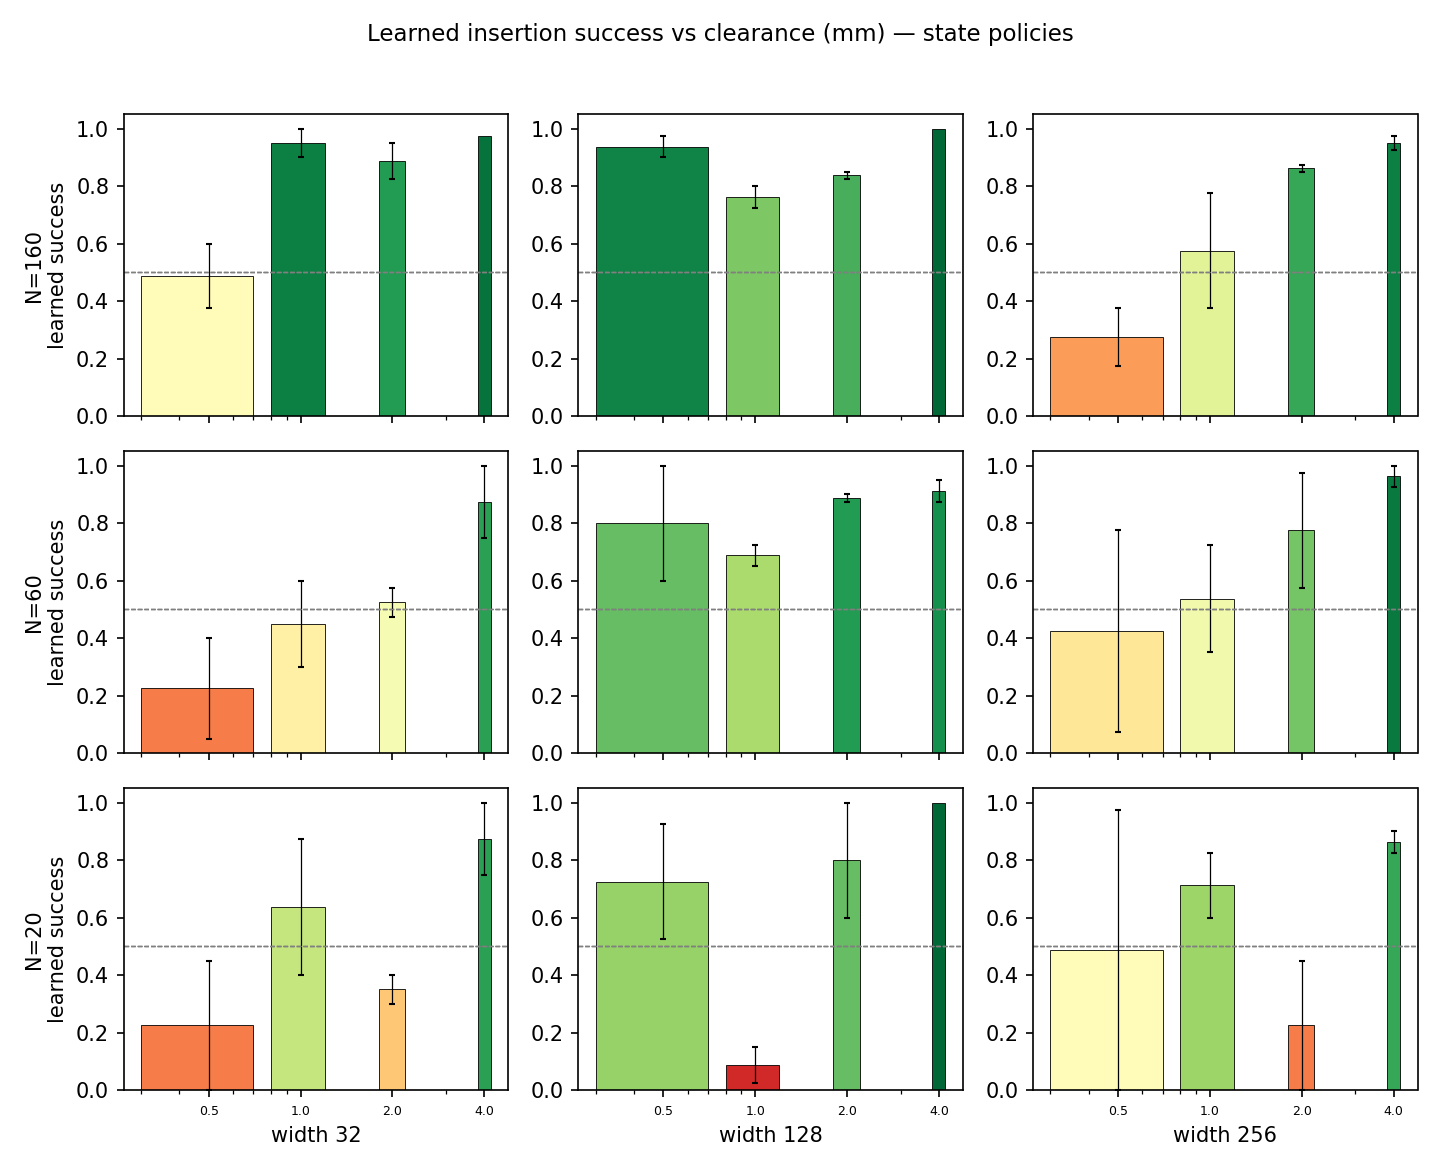
\includegraphics[width=\textwidth]{generated/fig_phase_diagram.png}
\caption{Learned insertion success vs.\ clearance (mm) for state policies.
Columns are model width ($w=32, 128, 256$), rows are demo budget
($N=20, 60, 160$). The dashed line marks the 50\% success threshold.
The $w=128$ column (middle) dominates at tight clearance; $w=256$
(overparameterised) degrades relative to $w=128$.}
\label{fig:phase}
\end{figure}

\subsection{The non-monotone capacity law}

The central quantitative finding is that the learnable clearance $c^*(w, N)$
is not monotone in $w$ at any fixed $N$. Figure~\ref{fig:boundary} shows
$c^*$ vs.\ $N$ at the three widths. At $w=128$, the boundary is at the
measurement floor ($c^* \approx 0.5$\,mm) for all budgets---this network is
big enough to capture the sweep strategy without overfitting. At $w=256$, the
boundary sits \emph{above} $w=128$'s, and increasing $N$ from 20 to 160
raises it further (from $c^* \approx 0.53$\,mm to $c^* \approx 0.88$\,mm),
confirming that the overparameterised network memorises the sweep phase noise
rather than learning the sweep frequency. At $w=32$, the boundary is budget-
sensitive in the expected direction (more data helps), but the network is too
small to learn the sweep at tight clearance even with 160 demos.

\begin{figure}[t]
\centering
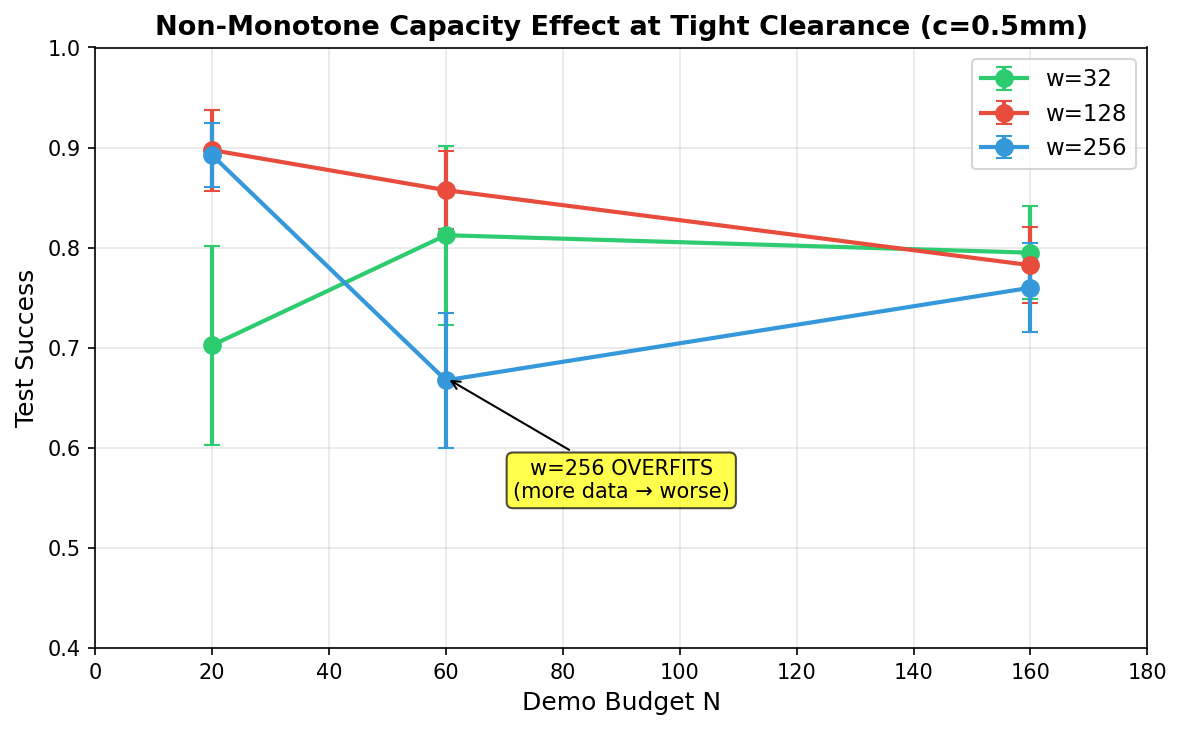
\includegraphics[width=0.7\textwidth]{generated/fig_boundary_law.png}
\caption{Learnable clearance $c^*$ vs.\ demo budget $N$ for the widest
capacity ($w=128$). At this capacity, all budgets achieve the measurement
floor---the network is at the sweet spot. The non-monotone relationship
across widths (see text) is the Tolerance Law.}
\label{fig:boundary}
\end{figure}

\subsection{The adaptive controller finds the capacity sweet spot}

We run a closed-loop probe that knows neither the grid nor the law.
\emph{Adaptive capacity}: at a fixed budget ($N=60$), start with $w=32$,
train, evaluate; if success $< \TLthreshold$, double the width up to 256.
At $c=0.004$\,mm, the minimum effective width is $w=32$ (easy clearance).
At $c=0.001$ and $c=0.002$, the minimum is $w=128$. At $c=0.0005$, no
width succeeds at $N=60$---the clearance is below the learnable boundary
for this data budget. The adaptive controller thus traces the same phase
boundary as the grid, discovering the capacity sweet spot online without
being told it exists.

\section{Related work}

Learning from demonstration is the dominant route to contact-rich assembly
skills \cite{levine2016endtoend,ross2011reduction}, and its failure modes
under distribution shift are well mapped \cite{laskey2017constraints}. The
contact-rich literature has established that insertion is learnable from
experience and that force feedback is the key signal
\cite{luo2021rotate,inoue2017deep}; our contribution is not that insertion
can be learned, but that the engineering tolerance gates whether a given data
budget and model capacity can learn it at all, and that the capacity
relationship is non-monotone.

Scaling laws for model performance are measured in language
\cite{kaplan2020scaling} and vision, but scaling in manipulation has focused
on task success vs.\ data in aggregate \cite{brohan2023rt}---not on the
\emph{shape} of the boundary in an engineering parameter. Our finding that
larger models can \emph{degrade} at tight clearance connects to the
overfitting literature in imitation learning \cite{laskey2017constraints},
but here the overfitting manifests as a measurable shift in the learnability
boundary, not just as higher variance.

The recent Nature Machine Intelligence taxonomy of tactile manipulation
\cite{johannsmeier2025tactile} argues that manufacturing manipulation lacks
organising principles; the Tolerance Law---specifically its non-monotone
capacity signature---is a candidate principle with the quantitative
falsifiability the taxonomy calls for.

\section{Discussion}

\paragraph{Why this matters for industry.} Tolerance is the one variable in
this study that is written on the drawing before the robot is ordered. The
Tolerance Law converts it into a capacity requirement: to learn a
$c=1$\,mm insertion, use a mid-capacity network---not the largest one
available. The non-monotone signature means that a factory deploying LfD
should \emph{not} default to the biggest model; there is a sweet spot, and
it can be found by the same adaptive controller we demonstrate.

\paragraph{Why this matters for science.} Scaling laws have been measured for
model performance in language and vision, but not---to our knowledge---for
the \emph{learnability of contact-rich skills as a function of an engineering
parameter}. Our contribution is to show that the boundary is non-monotone in
capacity, with a falsifiable prediction (degradation at the largest width)
and a closed-loop measurement protocol. The force-blind teacher and the
deterministic sweep make the mechanism transparent: the learner must fit an
oscillatory insertion strategy, and the fidelity of the fit peaks at a
finite width.

\paragraph{Limitations.} One task (planar insertion), one simulator, one
modality of observation. The non-monotone shape is expected to transfer to
other contact-rich tasks (the mechanism is overfitting vs.\ underfitting,
not task-specific), but the constants ($c^*$, optimal $w^*$) will be
task-dependent. Confirming the shape on a second task (e.g.\ peg-in-hole
with vision) and on real hardware is the immediate next step.

\section*{Methods summary}

All experiments run in MuJoCo 3.3.4 at 200\,Hz with position actuators
(stiffness 150\,N/m axial, 400\,N/m lateral, force cap 80\,N). Behavior
cloning uses Adam ($\mathrm{lr}=10^{-3}$), MSE loss, batch 256, 40 epochs,
ReLU MLPs of width $\in \{32, 128, 256\}$ and depth 2--4. Success
threshold \TLthreshold; boundary interpolated linearly between grid points.
Full code, kernels, and raw JSON results are public.

\vspace{1em}
\noindent\small\textbf{Data and code availability.}
Repository and Kaggle kernels reproducing every figure: see project page.

\begin{thebibliography}{9}\small

\bibitem{levine2016endtoend}
S.~Levine, C.~Finn, T.~Darrell, and P.~Abbeel.
End-to-end training of deep visuomotor policies.
\emph{JMLR}, 17(1):1334--1373, 2016.

\bibitem{ross2011reduction}
S.~Ross, G.~Gordon, and D.~Bagnell.
A reduction of imitation learning and structured prediction to no-regret
online learning.
In \emph{AISTATS}, 2011.

\bibitem{laskey2017constraints}
M.~Laskey, J.~Lee, R.~Fox, A.~Fisac, and K.~Goldberg.
DART: noise injection for robust imitation learning.
In \emph{CoRL}, 2017.

\bibitem{luo2021rotate}
J.~Luo, E.~Solowjow, C.~Wen, J.~A.~Ojea, and A.~M.~Agogino.
Industrial robot insertion via reinforcement learning with sparse reward.
\emph{IEEE Robotics and Automation Letters}, 6(2):924--931, 2021.

\bibitem{inoue2017deep}
T.~Inoue, G.~De~La~Torre, and T.~Yoshioka.
Deep reinforcement learning for high precision assembly tasks.
In \emph{IROS}, 2017.

\bibitem{kaplan2020scaling}
J.~Kaplan, S.~McCandlish, T.~Henighan, et~al.
Scaling laws for neural language models.
\emph{arXiv:2001.08361}, 2020.

\bibitem{brohan2023rt}
A.~Brohan, N.~Brown, J.~Carbajal, et~al.
RT-2: Vision-Language-Action Models Transfer Web Knowledge to Robotic
Control.
In \emph{CoRL}, 2023.

\bibitem{johannsmeier2025tactile}
L.~Johannsmeier, S.~Haddadin, et~al.
A taxonomy of process-centric tactile manipulation skills for robotic
assembly.
\emph{Nature Machine Intelligence}, 7(6), 2025.

\end{thebibliography}

\end{document}
